\documentclass[11pt,a4paper]{article}

\usepackage[T1]{fontenc}
\usepackage[utf8]{inputenc}
\usepackage{lmodern}
\usepackage[a4paper,margin=1in]{geometry}
\usepackage{amsmath,amssymb}
\usepackage{booktabs}
\usepackage{graphicx}
\usepackage{subcaption}
\usepackage{float}
\usepackage{hyperref}
\usepackage{xcolor}
\usepackage{enumitem}

\hypersetup{
  colorlinks=true,
  linkcolor=blue,
  citecolor=blue,
  urlcolor=blue
}

\title{Toy VELO Track Characterisation Study\\\large Derived from \texttt{characterisation.ipynb}}
\author{Quantum Track Reconstruction}
\date{\today}

\begin{document}
\maketitle

\begin{abstract}
This document summarises the workflow and analysis in
\texttt{Toy\_Characterisation/characterisation.ipynb}. The study evaluates
segment-pair angle behaviour, track reconstruction quality, and scaling trends
for a toy VELO model under varying event sizes, scattering strengths, and
angular phase-space settings. The key tuning parameter is the segment-pair
acceptance threshold $\varepsilon$, computed from detector and physics
uncertainties.
\end{abstract}

\section{Objectives}
The notebook performs five main tasks:
\begin{enumerate}[leftmargin=1.5em]
  \item Build reusable event-generation and angle-analysis helpers.
  \item Solve reconstruction on a clean event and validate truth--reco matching.
  \item Characterise pairwise segment-angle distributions on 10-event and
  100$\times$50-event ensembles.
  \item Run a parametric scan versus event size for multiple scattering and
  generation-angle settings.
  \item Produce acceptance histograms comparing true and false segment pairs.
\end{enumerate}

\section{Setup and Definitions}
\subsection{Geometry and Event Model}
A planar detector geometry is generated with evenly spaced modules:
\begin{itemize}[leftmargin=1.5em]
  \item Number of modules: configurable (clean-event baseline uses 5).
  \item First module position: $z_{0}=100\,\mathrm{mm}$.
  \item Module spacing: $\Delta z = 33\,\mathrm{mm}$.
  \item Half-widths: $l_x=l_y=50\,\mathrm{mm}$.
\end{itemize}

Events are generated with primary vertices and charged pion tracks, with
configurable angular bounds $\phi_{\max}$ and $\theta_{\max}$.

\subsection{Hamiltonian Acceptance Scale}
The acceptance threshold is computed as
\begin{equation}
\varepsilon = \sqrt{2\theta_s^2 + 12\theta_r^2 + 2\theta_{\min}^2},
\end{equation}
with
\begin{equation}
\theta_s = s\,\sigma_{\mathrm{scatt}},
\qquad
\theta_r = \arctan\!\left(\frac{s\,\sigma_{\mathrm{res}}}{\Delta z}\right),
\end{equation}
where $s$ is a sigma scale factor (default $s=3$ in this notebook).

For the clean-event baseline:
\begin{itemize}[leftmargin=1.5em]
  \item $\sigma_{\mathrm{res}}=0$,
  \item $\sigma_{\mathrm{scatt}}=10^{-4}\,\mathrm{rad}$,
  \item $\Delta z=33\,\mathrm{mm}$,
  \item $s=3$,
\end{itemize}
which gives approximately
\begin{equation}
\varepsilon \approx 4.24\times 10^{-4}\,\mathrm{rad}
\approx 0.424\,\mathrm{mrad}.
\end{equation}

\subsection{Segment-Pair Angle Definition}
The measured angle is the angle between consecutive segments sharing a middle
hit, \emph{not} the angle to the beam axis. For hits
$\mathbf{h}_{k-1},\mathbf{h}_k,\mathbf{h}_{k+1}$:
\begin{equation}
\alpha_k = \arccos\!\left(
\frac{(\mathbf{h}_{k}-\mathbf{h}_{k-1})\cdot(\mathbf{h}_{k+1}-\mathbf{h}_{k})}
{\lVert \mathbf{h}_{k}-\mathbf{h}_{k-1} \rVert
 \lVert \mathbf{h}_{k+1}-\mathbf{h}_{k} \rVert}
\right).
\end{equation}
A pair is labelled \textbf{true} only when all three hits lie on the same truth
track; otherwise it is \textbf{false}.

\section{Pipeline Summary}
\subsection{Caching and Persistence}
The notebook uses persistent storage under
\texttt{characterisation\_outputs/} to avoid recomputing expensive studies:
\begin{itemize}[leftmargin=1.5em]
  \item clean event pipeline,
  \item 10-event batch,
  \item 100$\times$50 angle distributions,
  \item parametric scan outputs,
  \item acceptance histogram study.
\end{itemize}
A \texttt{FORCE\_RECOMPUTE} switch controls regeneration.

\subsection{Clean Event Reconstruction}
A clean event with 3 tracks and 5 modules is generated, solved with
\texttt{SimpleHamiltonianFast}, then reconstructed with threshold
\begin{equation}
\text{baseline} = \frac{\delta}{\delta+\gamma},
\qquad
\text{threshold} = \frac{1+\text{baseline}}{2},
\end{equation}
using $\gamma=1.5$ and $\delta=1.0$.

Validation is performed with \texttt{EventValidator} using purity cut
\texttt{purity\_min=0.7}, reporting event metrics and per-track labels
(primary/ghost/clone).

\subsection{Multi-Event Studies}
\paragraph{10-event varying occupancy.}
Track counts are scanned over
\([2,3,4,5,6,3,4,5,2,4]\), with per-event summaries and overlaid truth/reco
plots.

\paragraph{100 events $\times$ 50 tracks.}
Large-sample true/false segment-angle distributions are accumulated and saved as
\texttt{angle\_distributions\_100x50.npz}.

\paragraph{Segment-level scan vs event size.}
Track multiplicity is scanned from 10 to 100 (step 10), with 5 repeats per
point, for:
\begin{itemize}[leftmargin=1.5em]
  \item scattering multipliers: $1\times$, $2\times$, $4\times$,
  \item angular settings: $\phi_{\max}=\theta_{\max}\in\{0.2,0.1,0.04\}$ rad.
\end{itemize}
For each configuration, the study records:
\begin{itemize}[leftmargin=1.5em]
  \item segment efficiency,
  \item segment false rate,
  \item counts of true/false segment pairs,
  \item counts of accepted true/false pairs with $\theta\le\varepsilon$.
\end{itemize}

\paragraph{Acceptance histograms.}
For each scattering-angle setting, 20 events at 50 tracks/event are generated,
with separate true/false histograms and normalised overlays.

\section{Metrics}
For each event or scan point, the notebook computes:
\begin{align}
\text{Segment efficiency} &=
\frac{N_{\text{true, accepted}}}{N_{\text{true pairs}}},\\
\text{Segment false rate} &=
\frac{N_{\text{false, accepted}}}{N_{\text{all accepted}}},
\end{align}
where acceptance is defined by $\theta\le\varepsilon$.

Scan summaries report means and standard errors across repeats.

\section{Figures and Outputs}
The notebook produces the following classes of visual outputs:
\begin{itemize}[leftmargin=1.5em]
  \item 3D truth event display for a clean event.
  \item Truth-vs-reconstructed event overlays.
  \item Per-event and aggregated true/false segment-angle histograms.
  \item 2$\times$2 metric panels versus event size for each angular setting.
  \item 3-column acceptance histogram panels (true/false/normalised overlay)
  for each scattering setting.
\end{itemize}

If the PNG exports already exist, include them directly. Two known examples in
this folder are shown below.

\begin{figure}[H]
  \centering
  \begin{subfigure}[b]{0.48\textwidth}
    \centering
    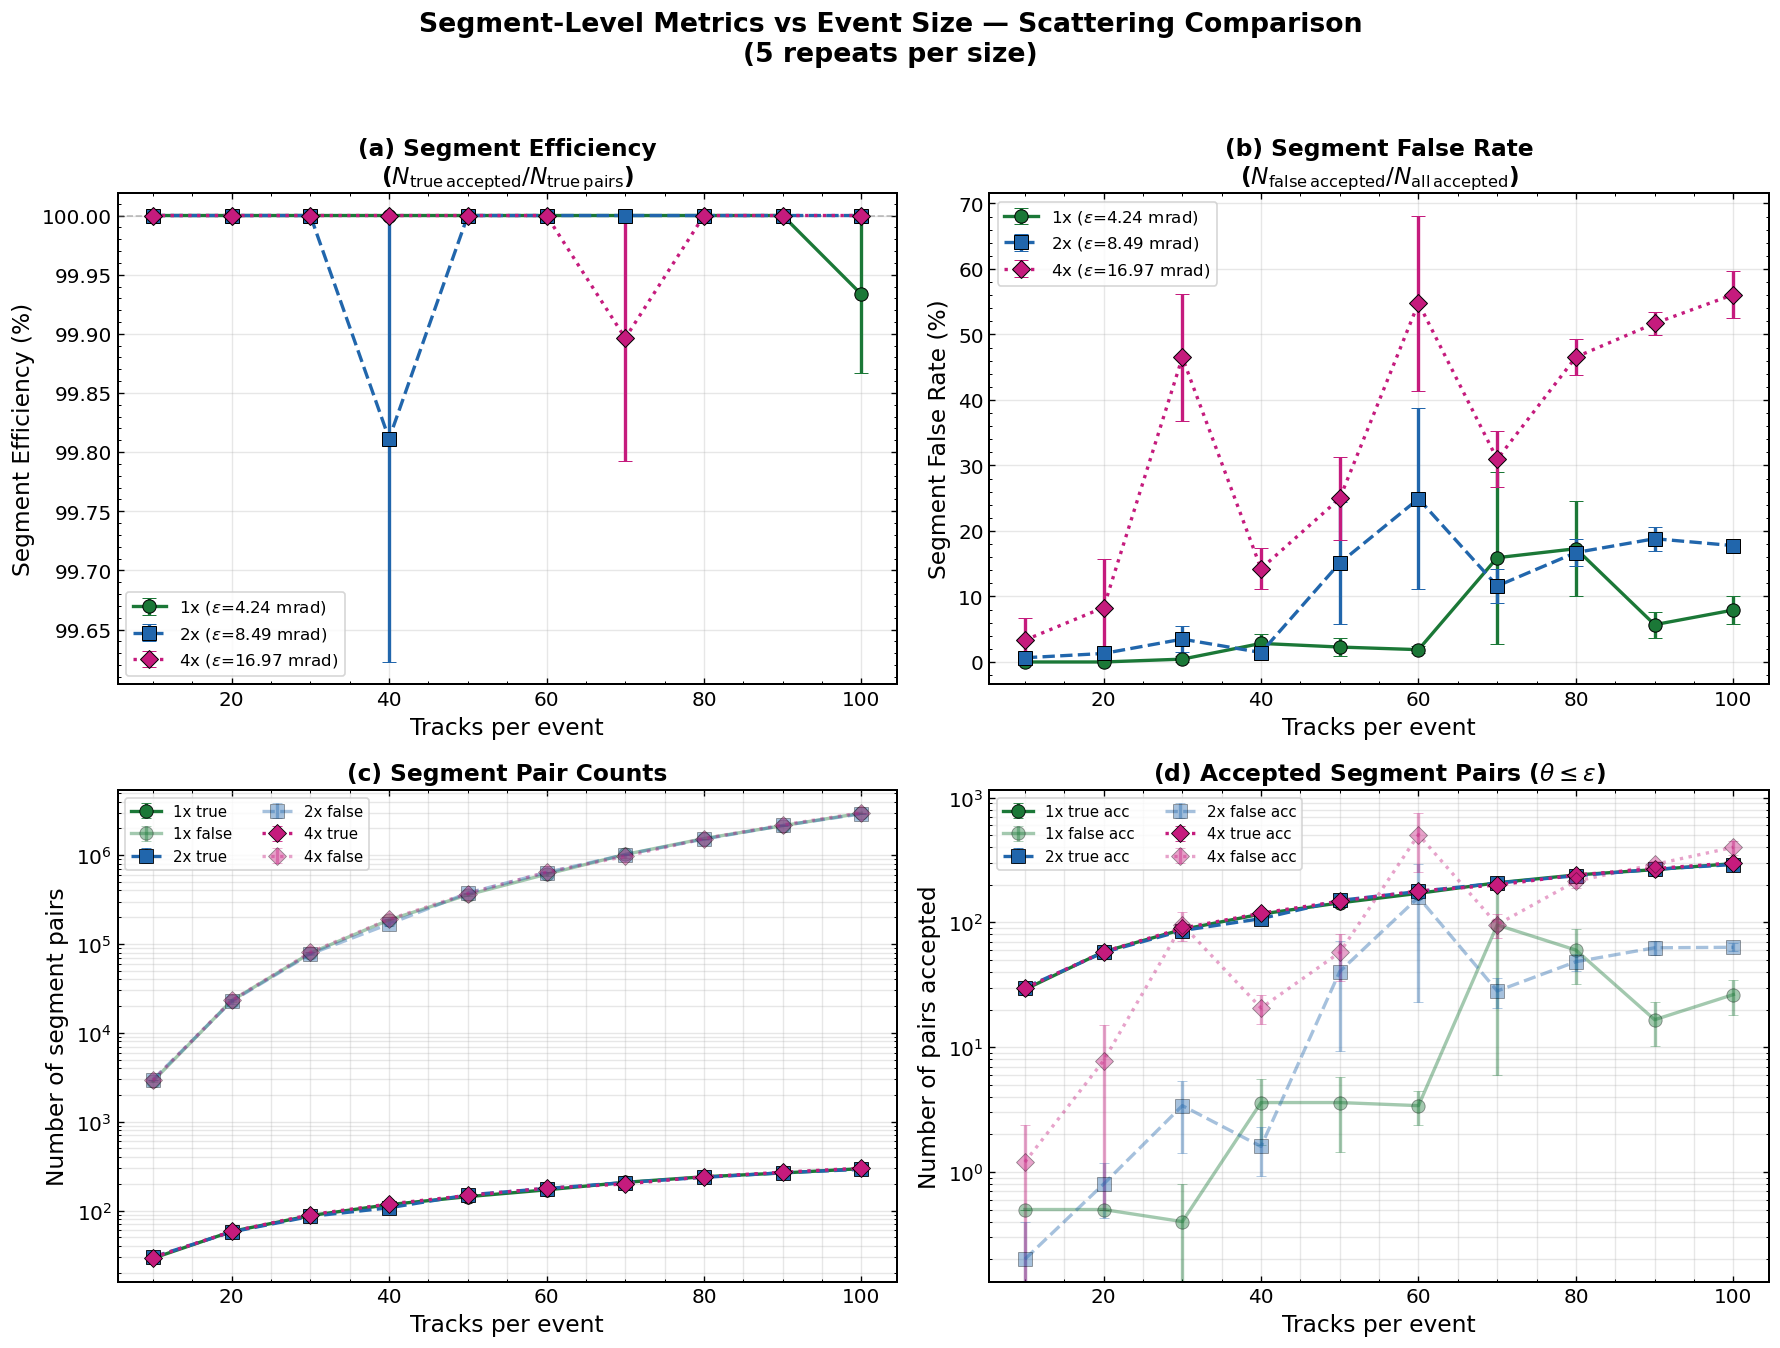
\includegraphics[width=\linewidth]{seg_eff_1mrad.png}
    \caption{Example segment-efficiency style output.}
  \end{subfigure}\hfill
  \begin{subfigure}[b]{0.48\textwidth}
    \centering
    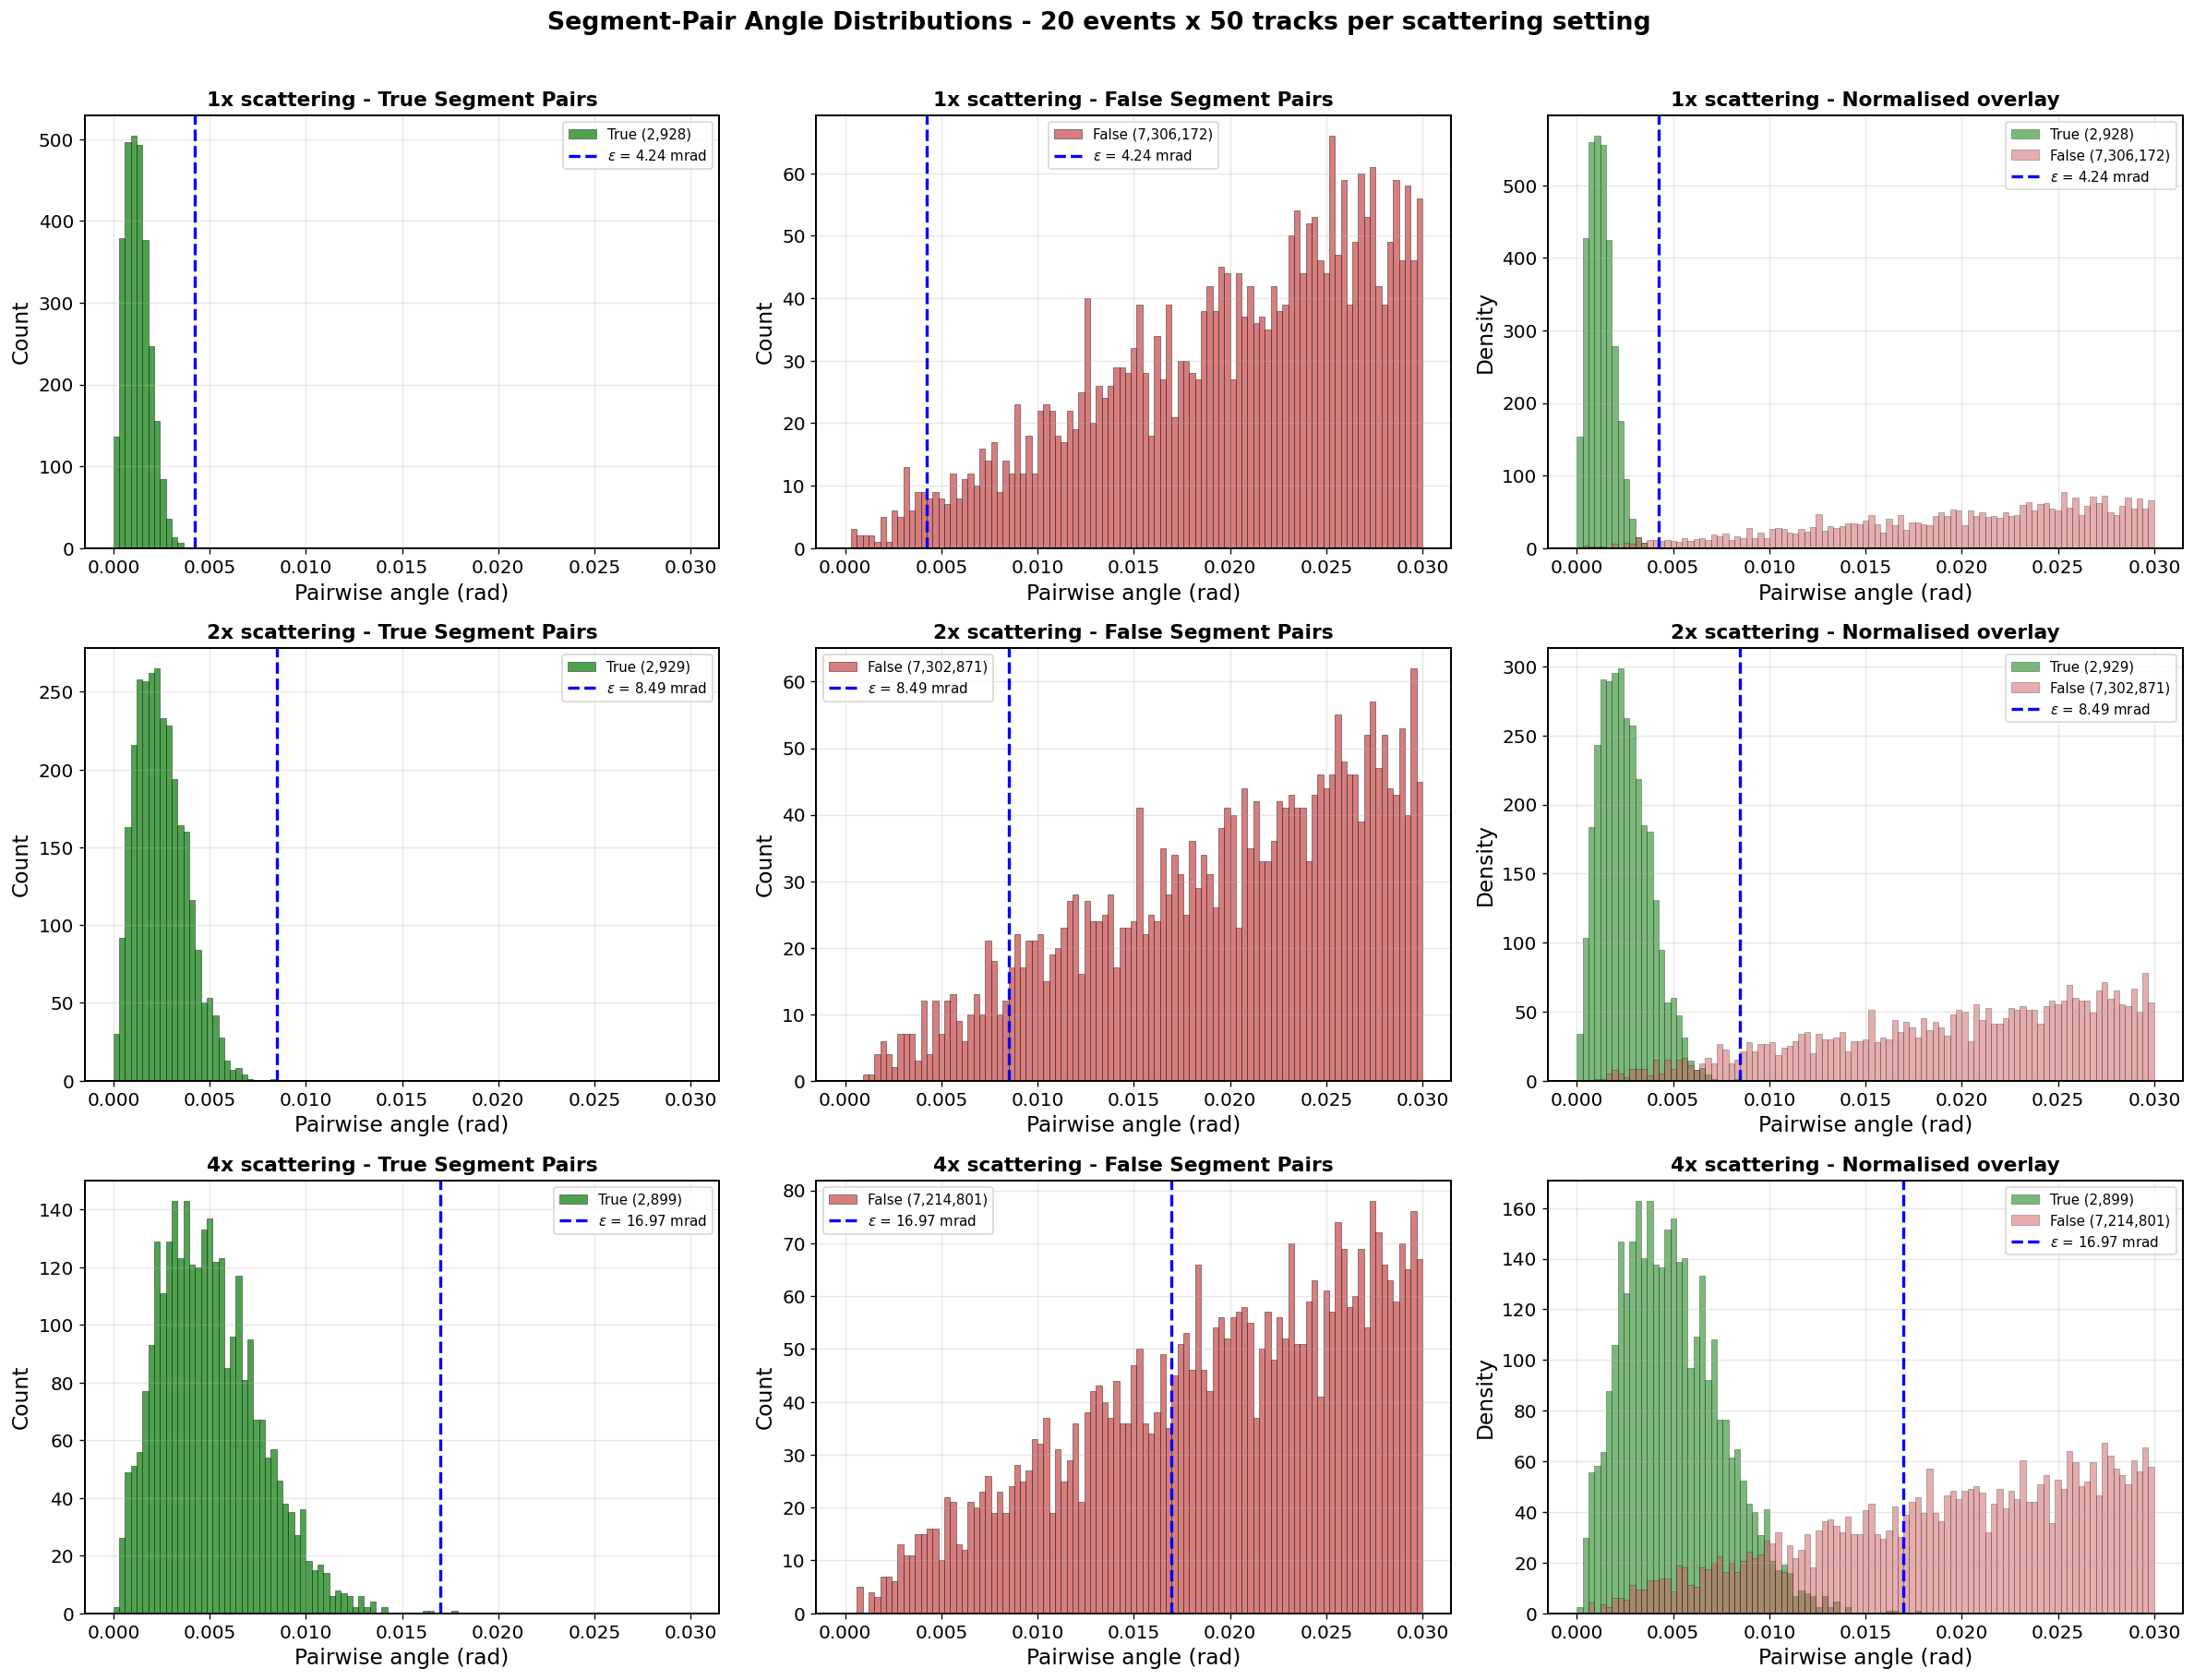
\includegraphics[width=\linewidth]{seg_hist_1mrad.png}
    \caption{Example segment-angle histogram output.}
  \end{subfigure}
  \caption{Representative figures exported in the study directory.}
\end{figure}

\section{Reproducibility Notes}
\begin{itemize}[leftmargin=1.5em]
  \item Core randomness comes from event generation; use fixed seeds if strict
  reproducibility is required.
  \item Cached outputs are reused unless \texttt{FORCE\_RECOMPUTE=True}.
  \item The parametric scans are computationally expensive and are designed to
  be checkpointed via persistence.
\end{itemize}

\section{How to Extend}
Recommended next extensions for this study:
\begin{itemize}[leftmargin=1.5em]
  \item Add uncertainty bands from bootstrap resampling in addition to standard
  error.
  \item Export all figure panels with deterministic filenames and add automatic
  LaTeX inclusion.
  \item Compare threshold strategies beyond fixed-sigma $\varepsilon$ (for
  example quantile-based acceptance).
\end{itemize}

\section{Conclusion}
The notebook implements a complete characterisation pipeline for toy VELO
segment-pair selection and reconstruction behaviour. Its main result is a
consistent framework to assess how acceptance thresholding, occupancy, angular
phase-space, and scattering jointly control efficiency--false-rate trade-offs.

\end{document}
